\chapter{Hardware Accelerator}

The Raspberry Pi 5 with an AI kit was chosen as the hardware to demonstrate the concept of edge computing.  
This decision was made based on recommendations from the advisors and the availability of the hardware.  
The market analysis confirms this choice.  
The hardware accelerator in the AI kit is produced by Hailo \cite{hailo}.  

Generally, a hardware accelerator is used to compute neural networks, similar to how a GPU is used for graphics processing.  
Hailo is a company that produces hardware accelerators.  
The AI kit uses the Hailo-8L entry-level accelerator.  
Hailo provides a pipeline to compile a network for execution on their hardware.  

First, we will examine the network compilation process, which must be done on a PC, preferably one with a GPU.  
Then, we will look at how to run the network on the edge.  

\section{Network Compilation}

As mentioned before, the network has to be precompiled on a PC.  
The application designed for this task is called the \Acrfull{dfc}.  

\subsection{Dataflow Compiler  
\label{section:dfc}}  

To use the \acrshort{dfc}, a PyTorch or TensorFlow model must be converted to ONNX or TensorFlow Lite.  
Information and images are taken from the Hailo Dataflow Compiler User Guide \cite{hailo_dataflow_compiler}.  
The \acrshort{dfc} then compiles the model to a \Acrfull{hef} by executing the following steps:  

\begin{enumerate}
    \item Full Precision Optimization
    \item Quantization Optimization
    \item Compilation
\end{enumerate}

In the full precision optimization step, the ONNX file is first compiled into a \acrfull{har} file, a file type defined by Hailo.  
This step also can include changes to the model in the floating-point precision domain, such as Equalization \cite{meller2019same}, \acrshort{tse} \cite{Vosco_2021_ICCV}, and pruning.  

In the quantization optimization step, the model is compressed.  
This means that the model is converted from floating-point to integer.  
Weights are compiled to either 4, 8, or 16 bits, while activations are compiled to 8 or 16 bits.  
Which quantization is applied is handled through a model script.  
In that script, the amount of quantized weights can be specified.  
It is also possible to target specific layers through the model script.  
Additionally, preprocessing steps can be added to the model script, such as resizing the input or converting the input from RGB to YUV.  

The result of this step is a quantized \acrshort{har} file.  
This file can then be compiled into a \acrshort{hef} file for use on Hailo hardware.  

\begin{figure}[!h]
    \centering
    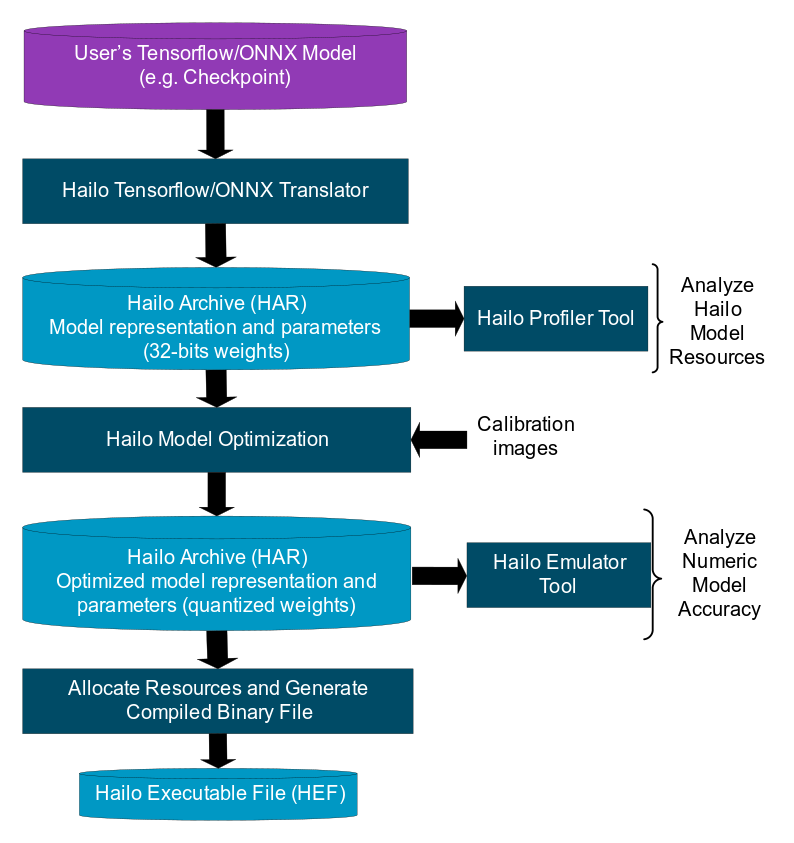
\includegraphics[width=\textwidth]{Images/Hardware/model_build_overview_with_onnx_and_hef_w_har.png}
    \caption{\Acrlong{dfc} overview \cite{hailo_dataflow_compiler}}
    \label{fig:hardware:dfcoverview}
\end{figure}

\subsection{Constraints}
At the time of this writing, the \acrshort{dfc} is not capable of compiling Transformers.  
This is an important limiting factor for this project.  
The best performance for CLIP is achieved with Vision Transformers as the image encoder.  
Fortunately, the visual encoding of CLIP can also be performed with ResNet (see \cref{crossmodalnetworks:sec:resnet}), a special form of \acrshort{cnn}'s.  

\section{Running on the Edge}

Hailo provides a library called TAPPAS, which is based on GStreamer.  
This library enables the use of a Hailo device within GStreamer pipelines to create intelligent video processing applications.  
The information for this section is taken from the TAPPAS User Guide.  

At present, there are two approaches to run a network on a Hailo device:  
one using GStreamer and another using a Python API.  
There are many different example applications available for various use cases.  
These examples can be found in the Hailo Model Zoo \cite{hailo_model_zoo} or in their repository for Raspberry Pi examples \cite{hailo_rpi5_examples}.  

\subsection{GStreamer Approach}

GStreamer is a framework for creating streaming media applications.  
It enables the design of any type of multimedia application, but it is not restricted to audio and video processing.  
The framework can process any kind of data flow.  

GStreamer consists of blocks that can be concatenated.  
To work with the Hailo hardware accelerator, some blocks in the pipeline are offloaded to the Hailo processor.  
A Python program is used to construct a string, which is then executed in a terminal.  
An example pipeline can be seen in \cref{fig:hardware:gstreamerpipeline}.  
More examples with code can be found in the TAPPAS User Guide.

\begin{figure}[!h]
    \centering
    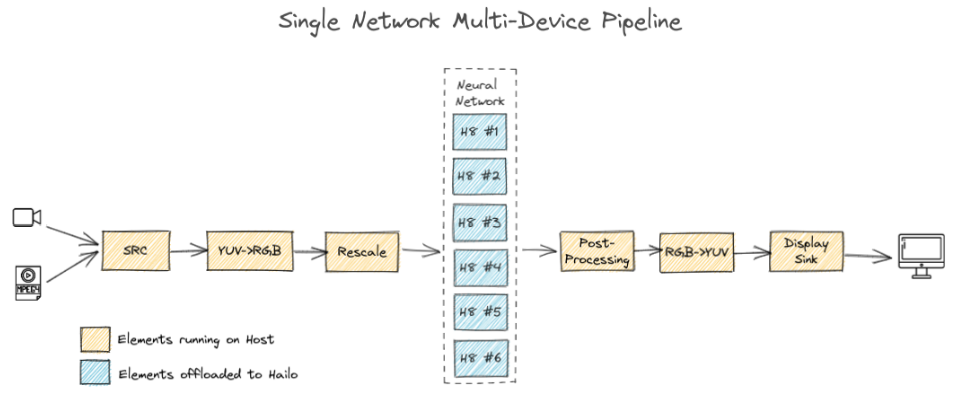
\includegraphics[width=\textwidth]{Images/Hardware/gstreamerExample.png}
    \caption{Example GStreamer pipeline from TAPPAS User Guide}
    \label{fig:hardware:gstreamerpipeline}
\end{figure}

\subsection{Python API Approach}

With the Python API approach, one can execute the entire inference in Python.  
This makes the program much simpler compared to the GStreamer approach.  
In Python, the Hailo hardware accelerator is treated as an object with dedicated functions for inference.  
It is important to note that Hailo swaps the input dimensions of the network.  
This means that the dimensions of the input to the network must be adjusted accordingly.  
Due to the complexity of the GStreamer approach, the Python API is used in this project.